\documentclass[margin=5pt]{standalone}
\usepackage{array}
\usepackage{amsmath,amssymb}
\usepackage{tikz}
\usetikzlibrary{arrows}
\usetikzlibrary{shapes}
\usetikzlibrary{backgrounds}
\usetikzlibrary{patterns}
\usetikzlibrary{positioning}
\usepackage{pgfplots}
\begin{document}
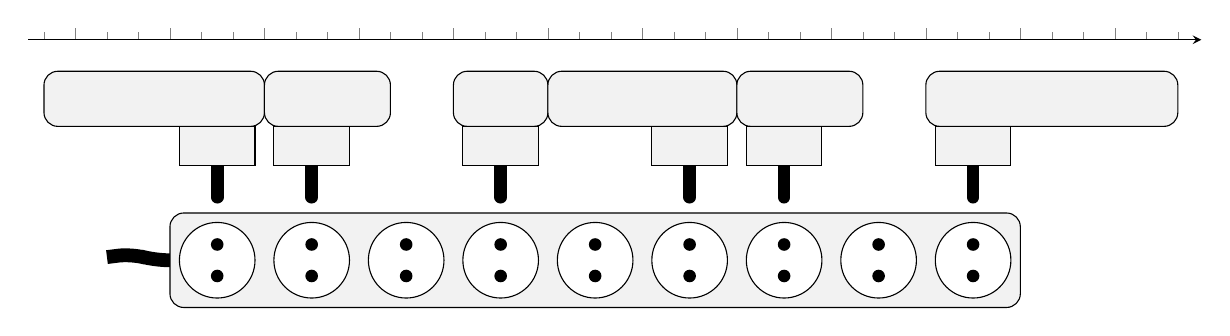
\begin{tikzpicture}[x=0.4cm,y=0.4cm]

	\begin{axis}[
		at={(0.4*-4.5cm,0.4*6cm)},
		grid style={opacity=0.25,color=black},
		x=0.4cm,y=0.4cm,
		axis lines=middle,
		axis y line=none,
		xmin=-4.5,
		xmax=32.75,
		ymin=0,
		ymax=0,
		xmajorticks=true,
		minor x tick num=2,
		xtick={-3.0,0.0,...,30.0},
		minor xtick={-4.0,...,32.0},
		xticklabels={,,},
		tick align=inside]%={-4.0,...,32.0}
	\end{axis}

	\newcommand{\socket}[1]{
	  \draw[rounded corners=5,fill=black!5] (0,-1.5) rectangle (3*#1, 1.5);
	  \draw[line width=5,rounded corners=5] (-2,0.1) -- (-1.2,0.2)--(-0.5,0)--(0,0);
	  \foreach \socket in {1,...,#1} {
		\draw[fill=white] (3*\socket-1.5,0) circle (1.2);
		\fill (3*\socket-1.5,0.5) circle (0.08cm);
		\fill (3*\socket-1.5,-0.5) circle (0.08cm);
	  }
	}

	\newcommand{\plug}[3]{
	  \draw[fill=black!5] (3*#1-1.2-1.5,4.25) rectangle (3*#1+1.2-1.5, 3);
	  \draw[line width=0.16cm] (3*#1-1.5,3) -- (3*#1-1.5, 2.5) edge[line cap=round] (3*#1-1.5, 2);
	  \draw[rounded corners=5,fill=black!5] (#2,4.25) rectangle (#3, 6);
	}

	\socket{9}
	\plug{1}{-4}{3}
	\plug{2}{3}{7}
	\plug{4}{9}{12}
	\plug{6}{12}{18}
	\plug{7}{18}{22}
	\plug{9}{24}{32}

\end{tikzpicture}
\end{document}
